%% Copyright 2015 M. Harland
  %
  % This work may be distributed and/or modified under the
  % conditions of the LaTeX Project Public License, either version 1.3
  % of this license or (at your option) any later version.
  % The latest version of this license is in
  %   http://www.latex-project.org/lppl.txt
  % and version 1.3 or later is part of all distributions of LaTeX
  % version 2005/12/01 or later.

%%%%%%%%%%
\documentclass[12pt,a4paper]{article}

\usepackage[left=2.5cm,right=2.5cm,top=1.0cm,bottom=2cm]{geometry}
\usepackage{placeins}

%\usepackage{graphicx}
%\usepackage{subcaption}
%\usepackage{amsmath}
%\parindent=1cm
%%%%%%%%%



%\marginparwidth = 0pt
%\hoffset = 0pt
%\oddsidemargin = 0pt
%\marginparsep = 0pt
%\voffset = 0pt

%\documentclass{amsproc}
%\documentclass[11pt,
%paper=a4,
%bibtotocnumbered,	  % Literaturverzeichnis ins Inhaltsverzeichnis
%liststotocnumbered,  % Alle Listen ins Inhaltsverzeichnis							
%DIV=calc,		  % führt die Satzspiegelberechnung neu aus
%oneside,		  % einseitiger Druck
%tablecaptionabove,	  % Tabellenüberschriften aktivieren
%BCOR=16mm,	  % Bindekorrektur
%headinclude,
%footinclude
%]{article}


%%%%
%\usepackage{fancyhdr}
%\usepackage{lipsum} % only for showing some sample text
%\fancyhf{} % clear all header and footers
%\renewcommand{\headrulewidth}{0pt} % remove the header rule
%\rfoot{\thepage}
%\pagestyle{fancy}
%\usepackage{indentfirst} % Красная строка
%%%%




\usepackage{amssymb}
\usepackage{amsmath}
\usepackage{graphicx}
\usepackage{color}
\def\x{{\bf x}}
\def\y{{\bf y}}
\newcommand{\XY}[1]{\textcolor{magenta}{X$\rightarrow$ Y: #1}}

\usepackage{mathrsfs,bbm}
\usepackage{comment}
\newcommand{\bm}[1]{\boldsymbol #1}
\newcommand{\lh}{\mbox{$\neg$}}
\newcommand{\rh}{\reflectbox{$\neg$}}
\usepackage{txfonts}
\DeclareSymbolFont{symbols}{OMS}{cmsy}{m}{n}
\DeclareSymbolFont{largesymbols}{OMX}{cmex}{m}{n}

%%%%%%%%%%%%%%%%%%%%%%%%%%%%%%%%%%%%%%%%%%%%%%%%
%Genaral math symbols
\newcommand{\TR}{\text{Tr}}
\newcommand{\BK}{{\bm k}}
\newcommand{\Vk}{{\bm k}}
\newcommand{\Ks}{{{\bm k}\sigma}}
\newcommand{\tb}{{\bar t}}
\newcommand{\myast}{{{}\hspace*{-0.1em}\ast\hspace*{-0.1em}{}}}
\newcommand{\mydagger}{{\dagger}}
\newcommand{\phdagger}{{\phantom{\dagger}\!}}
\newcommand{\bra}[1]{\langle{#1}|}
\newcommand{\ket}[1]{|{#1}\rangle}
\newcommand{\braket}[2]{\langle{#1}|{#2}\rangle}
\newcommand{\expval}[1]{\langle{#1}\rangle}
%%%%%%%%%%%%%%%%%%%%%%%%%%%%%%%%%%%%%%%%%%%%%%%%
%Contour calculus notation
\newcommand{\CS}{\mathcal{S}}
\newcommand{\ii}{^j}
\newcommand{\delC}{\delta_\CC}
\newcommand{\intC}{\int_\CC}
\newcommand{\tmin}{t_{\text{min}}}
\newcommand{\tmax}{t_{\text{max}}}
\newcommand{\CC}{\mathcal{C}}
\newcommand{\TC}{\mathcal{T}_{\CC}}
\newcommand{\gtrc}{\succ}
\newcommand{\lesc}{\prec}
%%%%%%%%%%%%%%%%%%%%%%%%%%%%%%%%%%%%%%%%%%%%%%%%
%Keldysh Green functions
\newcommand{\convz}{\ast}
\newcommand{\convi}{\bullet}
\newcommand{\convr}{\circ}
\newcommand{\ret}{{\text{R}}}
\newcommand{\adv}{{\text{A}}}
\newcommand{\mat}{{\text{\tiny M}}}
\newcommand{\tv}{{\makebox{$\neg$}}}
\newcommand{\vt}{{\reflectbox{$\neg$}}}
\newcommand{\les}{<}
\newcommand{\lar}{>}
%%%%%%%%%%%%%%%%%%%%%%%%%%%%%%%%%%%%%%%%%%%%%%%%
%misc
\newcommand{\ETAL}{{\em et al.}}
\newcommand{\Ucdyn}{{U_{\text{dyn}}}}
\newcommand{\sss}{_{\alpha\alpha'}}
\newcommand{\YY}{Y}
\newcommand{\KK}{K}
\newcommand{\pseudo}{\widetilde}
\newcommand{\cyles}{\prec}
\newcommand{\scell}{\text{scel}}
\newcommand{\pG}{\mathcal{G}}
%%%%%%%%%%%%%%%%%%%%%%%%%%%%%%%%%%%%%
%FK
\newcommand{\Gwnull}{Q}\newcommand{\Gweins}{R}
\newcommand{\gwnull}{q}\newcommand{\gweins}{r}
%%%%%%%%%%%%%%%%%%%%%%%%%%%%%%%%%%%%%
% for Mott Breakdown
\renewcommand{\dh}{dh}
\newcommand{\jd}{\Gamma_\text{\dh}}
\newcommand{\fth}{F_\text{th}}
\newcommand{\hopp}{{t^*}}
\renewcommand{\bar}{\overline}

%\input{defs}
\newcommand{\cis}{c_{i\sigma}}
\newcommand{\cisd}{c_{i\sigma}^\dagger}
\newcommand{\cs}{c_{\sigma}}
\newcommand{\csd}{c_{\sigma}^\dagger}
\newcommand{\cst}{c_{\sigma}(\tau)}
\newcommand{\csdtp}{c_{\sigma}^\dagger(\tau')}
\newcommand{\nup}{n_{\uparrow}}
\newcommand{\ndown}{n_{\downarrow}}
\newcommand{\nupt}{\nup(\tau)}
\newcommand{\ndownt}{\ndown(\tau)}
\newcommand{\nuptp}{\nup(\tau')}
\newcommand{\ndowntp}{\ndown(\tau')}
\newcommand{\nuptpp}{\nup(\tau'')}
\newcommand{\ndowntpp}{\ndown(\tau'')}
\newcommand{\nupti}{\nup(\tau_i)}
\newcommand{\nupta}{\nup(\tau_1)}
\newcommand{\ndownti}{\ndown(\tau_i)}
\newcommand{\ndownta}{\ndown(\tau_1)}
\newcommand{\nuptj}{\nup(\tau_j)}
\newcommand{\nuptb}{\nup(\tau_2)}
\newcommand{\ndowntj}{\ndown(\tau_j)}
\newcommand{\ndowntb}{\ndown(\tau_2)}
\newcommand{\nuptk}{\nup(\tau_k)}
\newcommand{\ndowntk}{\ndown(\tau_k)}
\newcommand{\Tr}{\text{Tr}}
\newcommand{\Hloc}{H_\text{loc}}
\newcommand{\Hhyb}{H_\text{hyb}}
\newcommand{\Hhybtwid}{\tilde{H}_\text{hyb}}
\newcommand{\fatx}{\mathbf{x}}
\newcommand{\fatX}{\mathbf{X}}
\newcommand{\fatk}{\mathbf{k}}
\newcommand{\fatK}{\mathbf{K}}
\newcommand{\fattildek}{\mathbf{\tilde{k}}}
\newcommand{\fattildex}{\mathbf{\tilde{x}}}
\newcommand{\fatt}{\mathbf{t}}
\newcommand{\fatg}{\mathbf{g}}
\newcommand{\fatG}{\mathbf{G}}
\newcommand{\fatbarG}{\mathbf{\overline{G}}}
\newcommand{\fatmathcalG}{\mathbf{\mathcal{G}}}
\newcommand{\fatSigma}{\mathbf{\Sigma}}
\newcommand{\vk}{{\mathbf{k}}}
\newcommand{\N}{{\mathbf{N}}}
\newcommand{\G}{{\mathbf{G}}}
\newcommand{\D}{{\mathbf{D}}}
\newcommand{\M}{{\mathbf{M}}}
\newcommand{\fatP}{{\mathbf{P}}}

\def\stau{\{ s_{i},\tau_{i}, x_i\}}
\def\staup{\{ s_{i}',\tau_{i}', x_i'\}}
\newcommand{\hyb}[2]{\Delta(\tau_{#1}^e-\tau_{#2}^s)}


\newcommand{\pa}{\partial}
\newcommand{\vphi}{\varphi}
\newcommand{\ve}{\varepsilon}
\newcommand{\up}{\uparrow}
\newcommand{\dw}{\downarrow}
\newcommand{\Vect}[1]{\mbox{\boldmath$#1$}}


% for introduction
\newcommand{\mb}[1]{\mathbf{#1}}
\newcommand{\mcl}[1]{\mathcal{#1}}
\newcommand{\al}{\alpha}
\newcommand{\be}{\beta}
\newcommand{\bz}{\bar{z}}
\newcommand{\e}{\epsilon}
\newcommand{\s}{\sigma}
\newcommand{\om}{\omega}
\newcommand{\la}{\lambda}
\newcommand{\bJ}{\bar{J}}
\newcommand{\brz}{\bar{z}}
\newcommand{\brq}{\bar{q}}
\newcommand{\vp}{\varphi}
\newcommand{\bvp}{\bar{\varphi}}
\newcommand{\tvp}{\tilde{\varphi}}
\newcommand{\hil}{\mcl{H}}
\newcommand{\vir}{\mathfrak{Vir}}
\newcommand{\no}{\nonumber}
\newcommand{\tr}{\mbox{Tr}}
\newcommand{\itl}{{\it l}}
\newcommand{\mbx}{\mathbf{x}}
\newcommand{\ihbar}{\frac{i}{\hbar}}



















%%%%
%\usepackage[utf8]{inputenc}
%\usepackage{graphicx} %includegraphics
%\usepackage{braket} %Bra and Ket
%\usepackage{amsmath} %mathcal etc
%\usepackage{natbib} %citep, citet, bib-style
%\usepackage[colorlinks]{hyperref}
%\newcommand{\mysubtitle}[1]{\section{#1}}
%\usepackage[usenames,dvipsnames]{xcolor}
%%%%
%\definecolor{persianplum}{rgb}{0.44, 0.11, 0.11}
%\definecolor{mulberry}{rgb}{0.77, 0.29, 0.55}
%\definecolor{maroon(html/css)}{rgb}{0.5, 0.0, 0.0}
%\definecolor{indigo(dye)}{rgb}{0.0, 0.25, 0.42}
\begin{document}
\title{Dynamical repulsion-attraction transition of doublons}
%\author{V.N. Valmispild}
\date{\today}
\maketitle
\tableofcontents
\section{Introduction}

Transport investigation in strongly correlated materials out of equilibrium is a convenient way of controlling their properties and can lead to discover unexpected physics. One manifestation of strong correlations is the Mott insulator.
Mott insulator is a clear example of strong correlations where doubly occupied sites play the role of carriers. This causes a big interest in the study of doublon dynamics in experimental and theoretical works due to development of the ultrafast time-resolved experimental techniques.
There are exist ways to change the number of doublons in such materials are doping or pumping of the sample by laser pulse. 

In work of [Hideo] described how the double occupancy changes with in the magnitude of the vector potential, which leads to a change in the sign of the Coulomb interaction. 

In this paper, we want to discuss how the doublone-doublone interaction depends on the magnitude of the external electric field. 





\FloatBarrier
\section{Model and method}
The Hamiltonian of the driven half-filled Hubbard model is
\begin{equation}
\begin{split}
H(t)&=\sum_{ij,\sigma}t_{ij}{\rm exp}{\left( -i\int_{{\bf R}_{j}}^{{\bf R}_{i}}d{\bf r} \cdot {\bf A}(t) \right)}c_{i \sigma}^{\dagger}c_{j \sigma}\\
&{+U{\sum_{i} \left(n_{i \uparrow}-\frac{1}{2}\right) \left(n_{i \downarrow}-\frac{1}{2} \right)}},
\end{split}
\end{equation}

where $t_{ij}$ are electron hopping amplitudes between sites $i$ and $j$, $c^\dagger_{i\sigma}$ the creation operator for an electron of spin $\sigma$ at site $i$, $U$ the on-site interaction, $n=c^\dagger c$ the number operator. Time-dependent double occupancy defined as $d(t)= \left\langle  {n}_{\uparrow}(t) {n}_{\downarrow}(t) \right\rangle $.  To solve the model we use the nonequilibrium dynamical mean field theory (DMFT) \cite{RevModPhys_NEDMFT} in combination with a weak coupling perturbative impurity solver (iterative perturbation theory (IPT)) \cite{RevModPhys_DMFT,Damping_of_BO}. We consider an 2D square lattice with dispersion law $\varepsilon({\bf k},t)=2t\left[{\rm cos}(k_x+A_x(t))+{\rm cos}(k_y+A_y(t))\right]$ and apply the electric field along the diagonal. In a gauge with pure vector potential $A(t)$, the electric field $E(t)=-\partial_t A(t)$ enters the calculation as a time-dependent shift of the noninteracting dispersion, $\epsilon_k\rightarrow \epsilon_{k-A(t)}$. We start at $t$ = 0 in the equilibrium state at inverse temperature $\beta$=5 and switch on the vector potential as it shown in Fig. \ref{fig:Pulse_21_10}.
\FloatBarrier



\FloatBarrier
\section{Shift of the Hubbard bands}

 
\begin{figure}[h!]
\begin{minipage}[h]{0.5\linewidth}
\center{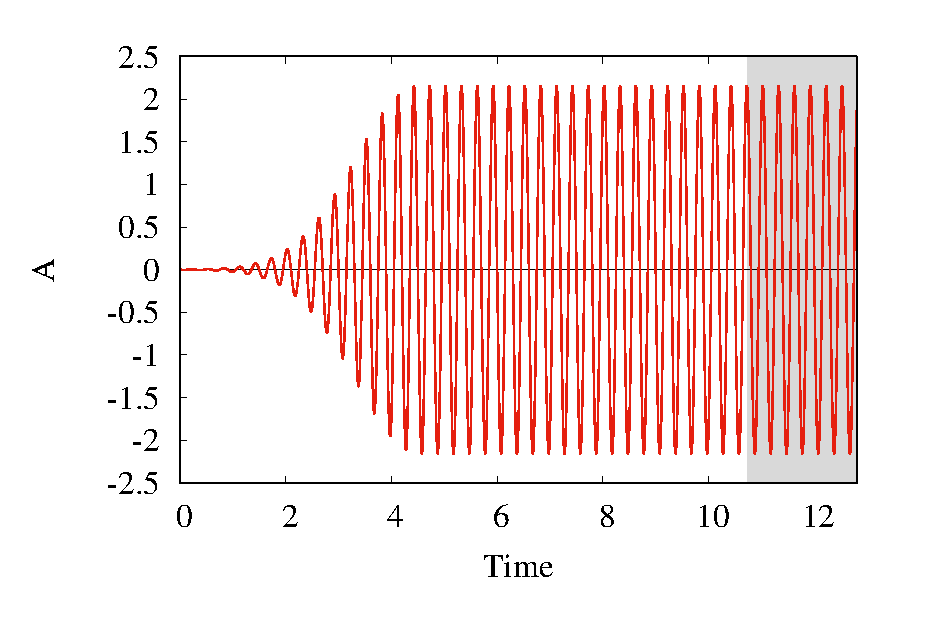
\includegraphics[width=1\linewidth]{./figure/Pulse_21.eps}} (a) \\
\end{minipage}
\hfill
\begin{minipage}[h]{0.5\linewidth}
\center{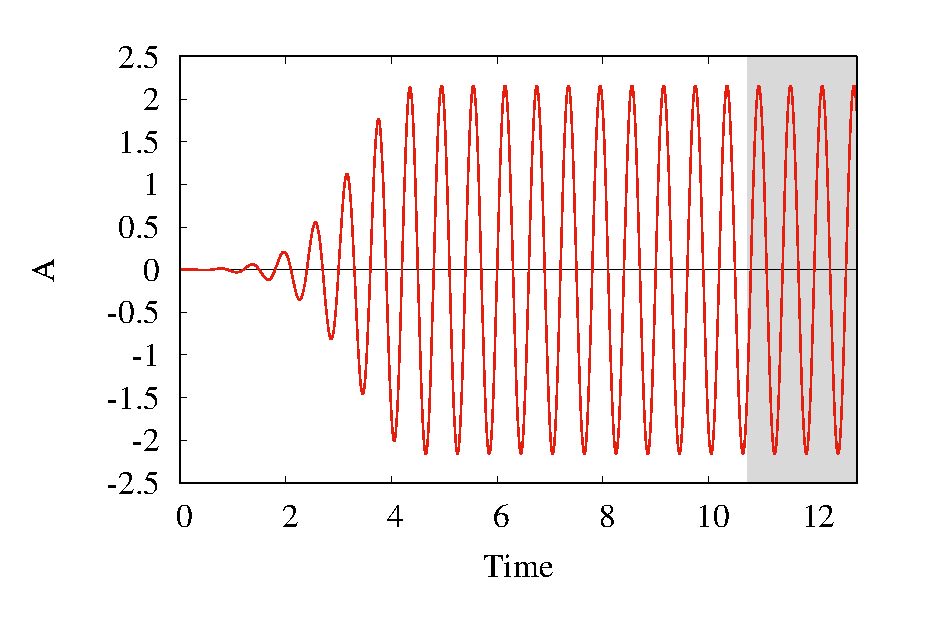
\includegraphics[width=1\linewidth]{./figure/Pulse_10.eps}} \\(b)
\end{minipage}
\caption{Pulse (a)21, (b)10.}
\label{fig:Pulse_21_10}
\end{figure}





\begin{figure}[h!]
\begin{minipage}[h]{0.5\linewidth}
\center{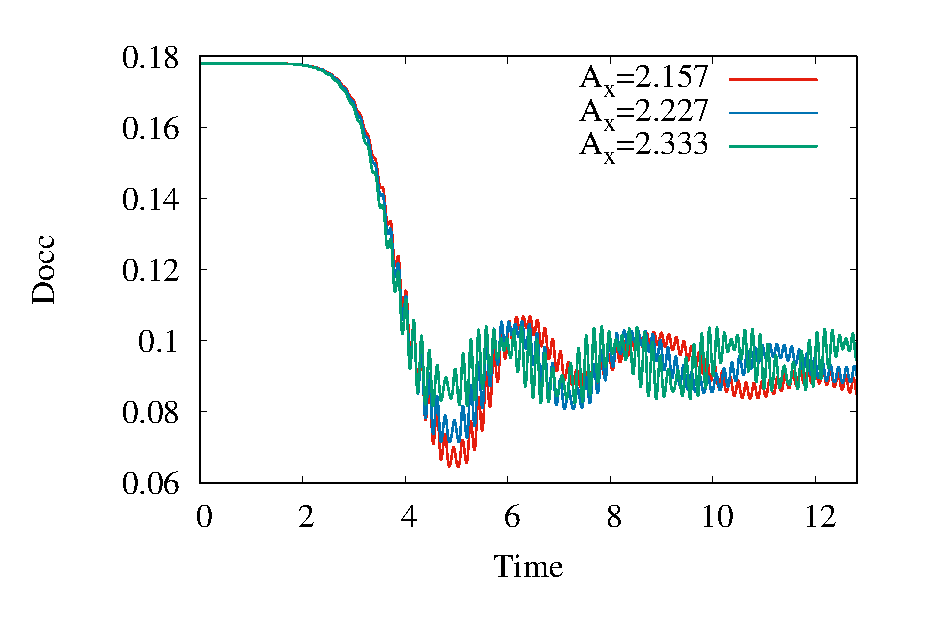
\includegraphics[width=1\linewidth]{./figure/docc_time_w21.eps}} (a) \\
\end{minipage}
\hfill
\begin{minipage}[h]{0.5\linewidth}
\center{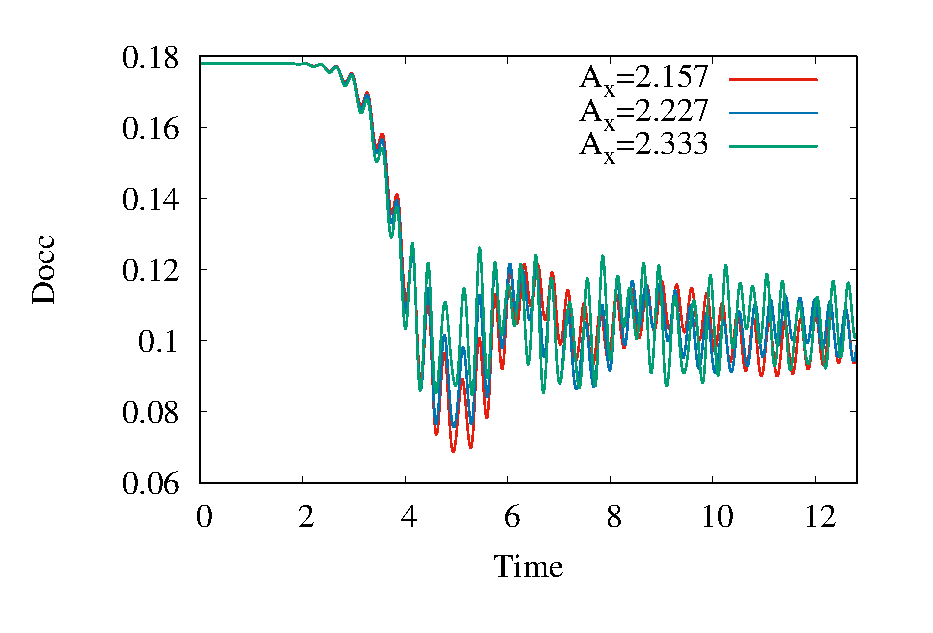
\includegraphics[width=1\linewidth]{./figure/docc_time_w10.eps}} \\(b)
\end{minipage}
\caption{docc}
\label{fig:docc time w21_10}
\end{figure}





\begin{figure}[h!]
\begin{minipage}[h]{0.5\linewidth}
\center{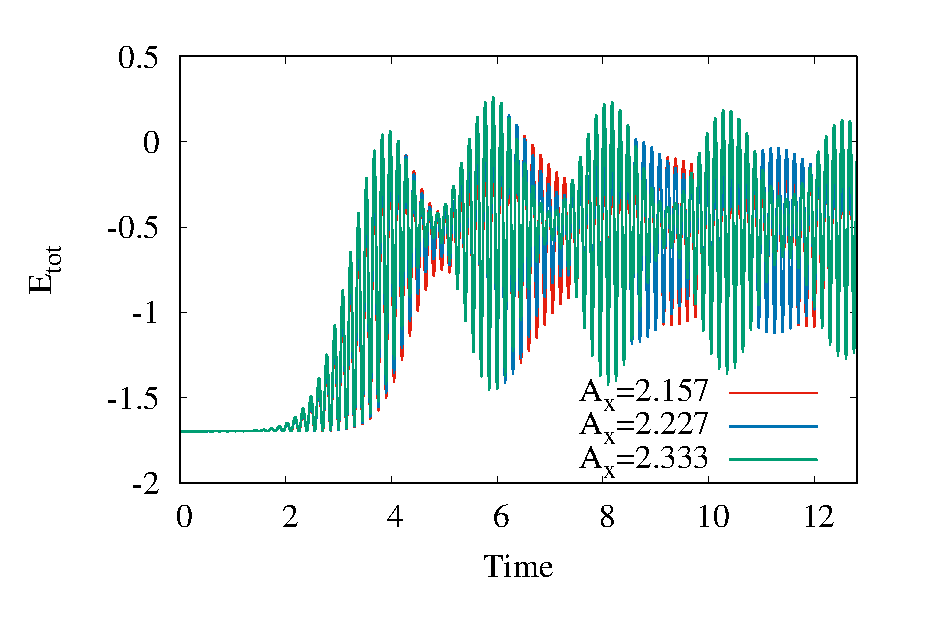
\includegraphics[width=1\linewidth]{./figure/Etot_time_w21.eps}} (a) \\
\end{minipage}
\hfill
\begin{minipage}[h]{0.5\linewidth}
\center{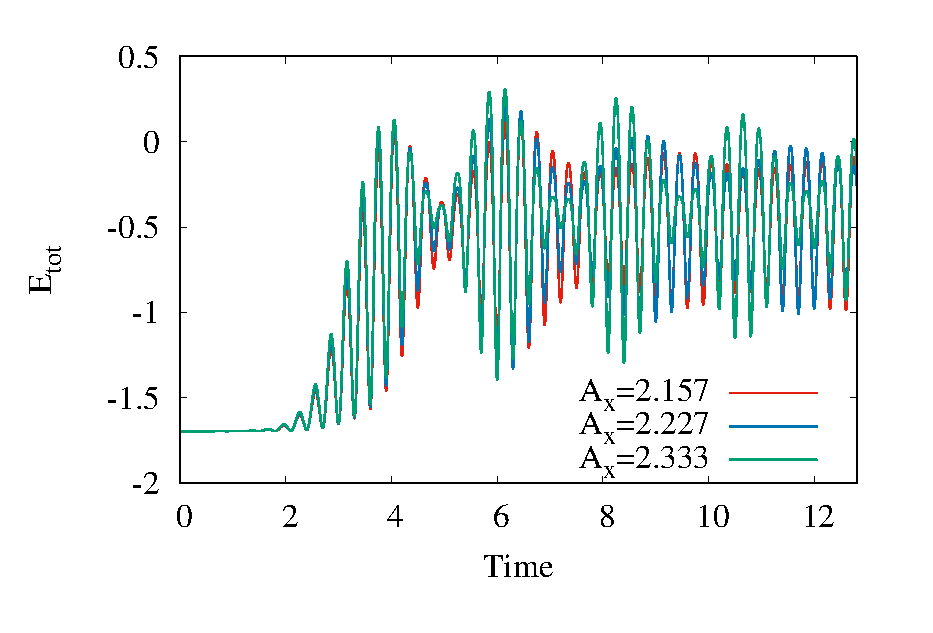
\includegraphics[width=1\linewidth]{./figure/Etot_time_w10.eps}} \\(b)
\end{minipage}
\caption{Etot}
\label{fig:Etot time w21_10}
\end{figure}




\begin{figure}[h!]
\begin{minipage}[h]{0.5\linewidth}
\center{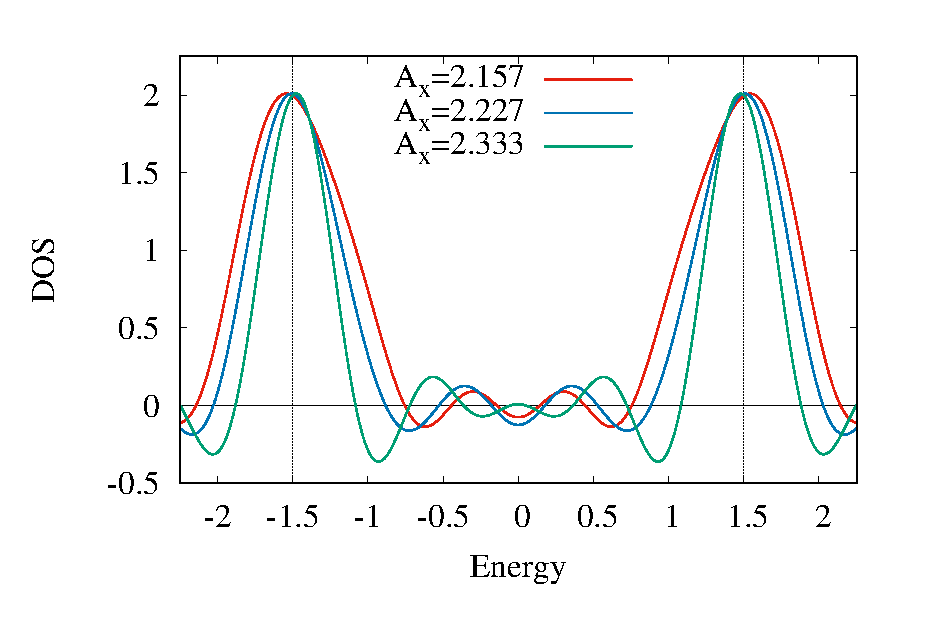
\includegraphics[width=1\linewidth]{./figure/DOS_21.eps}} (a) \\
\end{minipage}
\hfill
\begin{minipage}[h]{0.5\linewidth}
\center{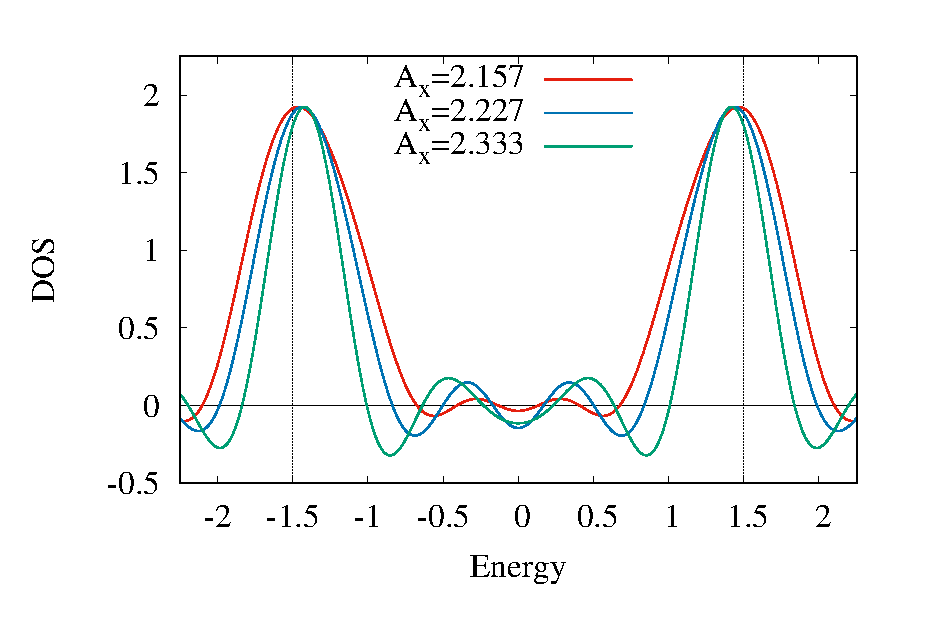
\includegraphics[width=1\linewidth]{./figure/DOS_10.eps}} \\(b)
\end{minipage}
\caption{DOS}
\label{fig:DOS w21_10}
\end{figure}



\begin{figure}[h!]
\begin{minipage}[h]{0.5\linewidth}
\center{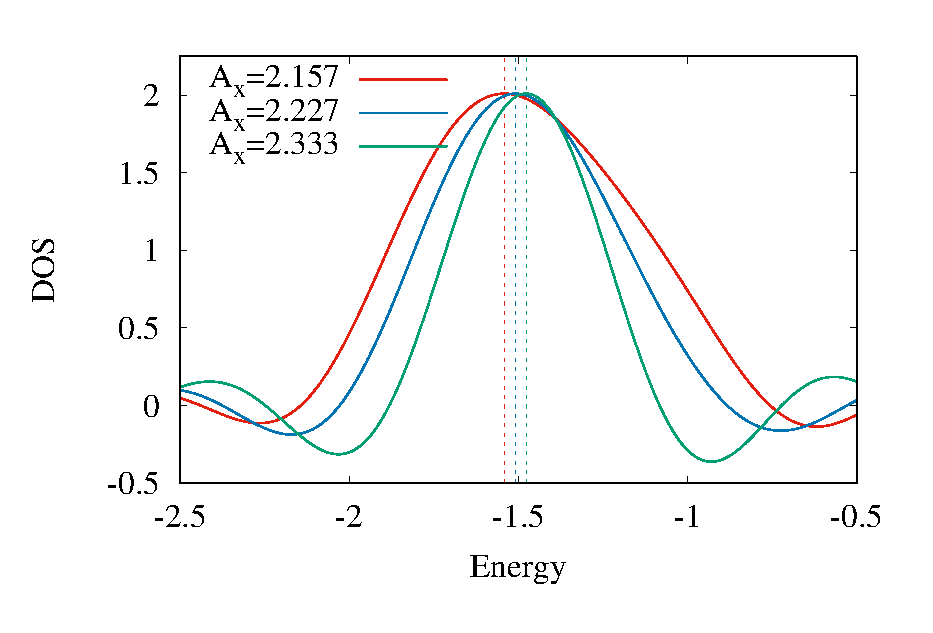
\includegraphics[width=1\linewidth]{./figure/DOS_21_small.eps}} (a) \\
\end{minipage}
\hfill
\begin{minipage}[h]{0.5\linewidth}
\center{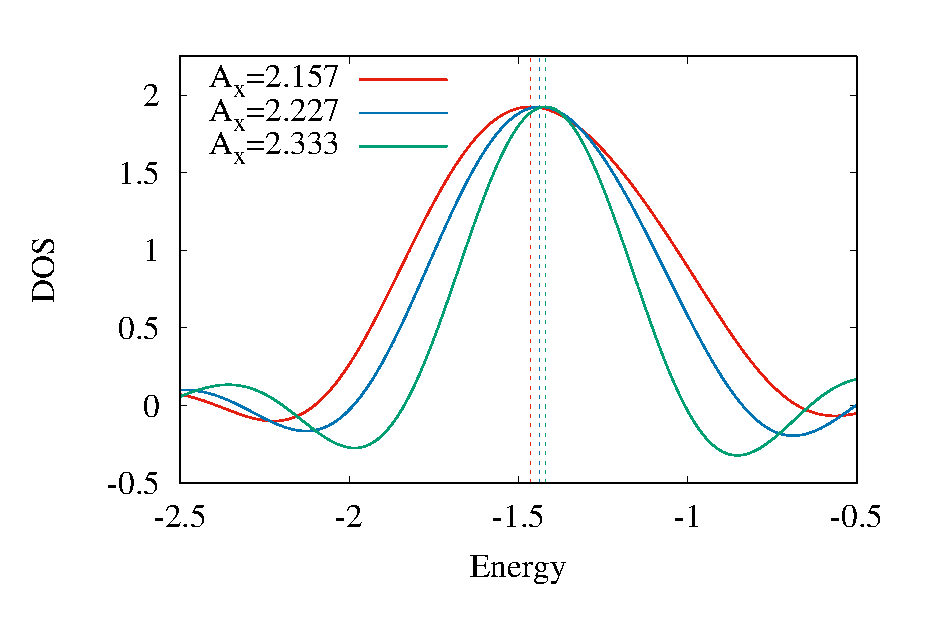
\includegraphics[width=1\linewidth]{./figure/DOS_10_small.eps}} \\(b)
\end{minipage}
\caption{DOS small}
\label{fig:DOS small w21_10}
\end{figure}





\begin{figure}[h!]
\begin{minipage}[h]{0.5\linewidth}
\center{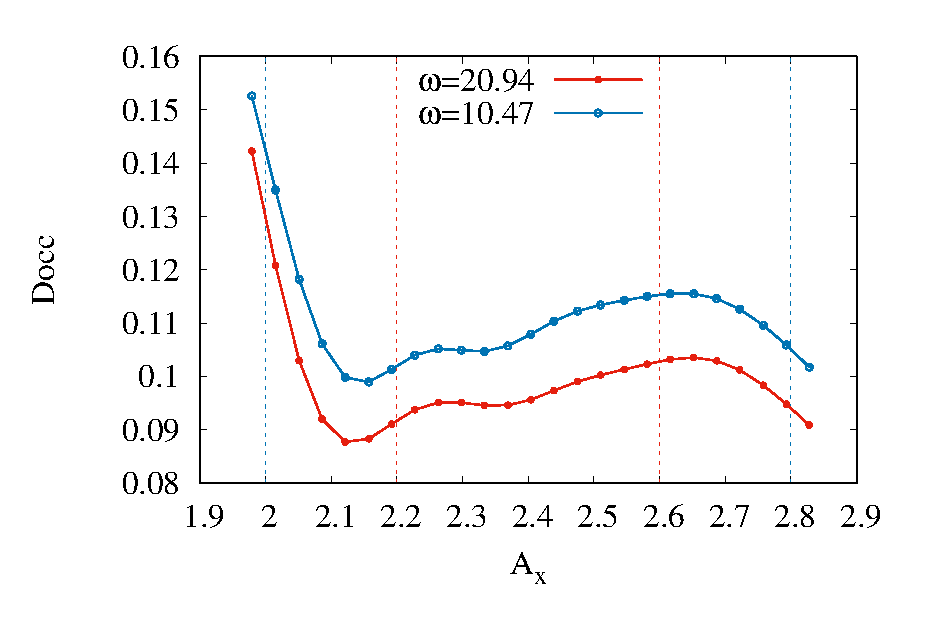
\includegraphics[width=1\linewidth]{./figure/docc.eps}} (a) \\
\end{minipage}
\hfill
\begin{minipage}[h]{0.5\linewidth}
\center{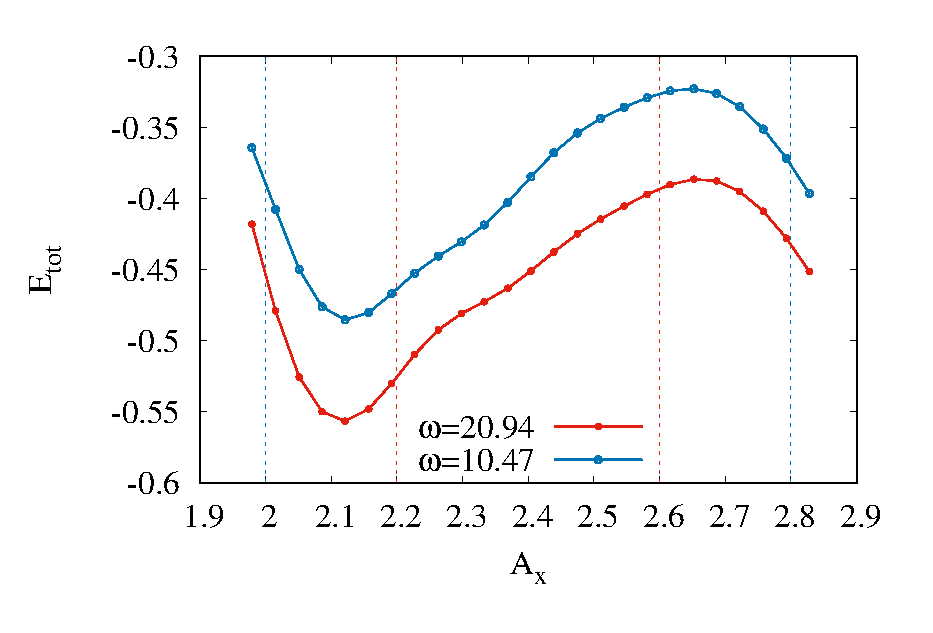
\includegraphics[width=1\linewidth]{./figure/E_tot.eps}} \\(b)
\end{minipage}
\caption{docc Etot}
\label{fig:docc_Etot}
\end{figure}






\begin{figure}[h!]
\begin{minipage}[h]{0.5\linewidth}
\center{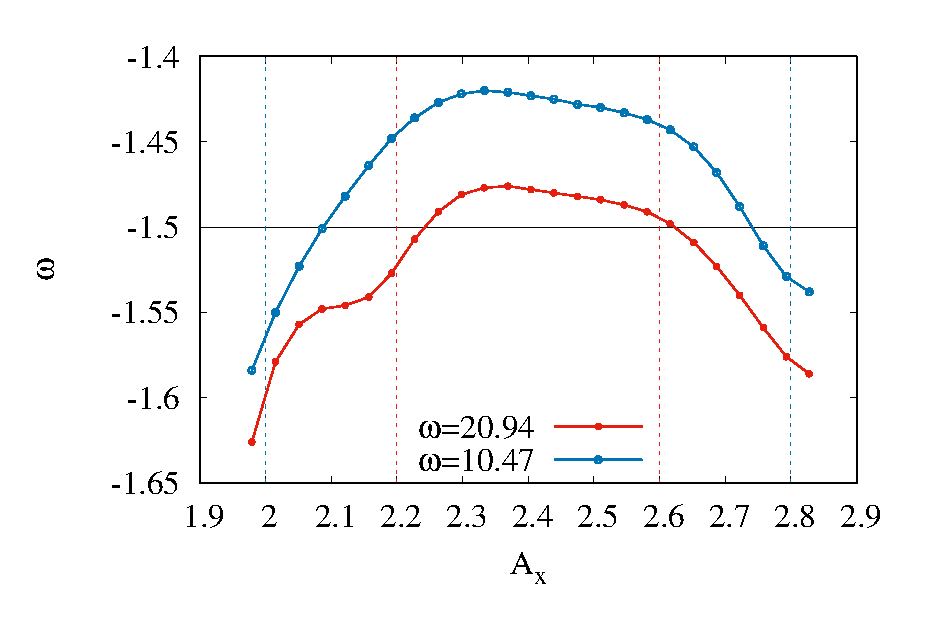
\includegraphics[width=1\linewidth]{./figure/omega.eps}} (a) \\
\end{minipage}
\hfill
\begin{minipage}[h]{0.5\linewidth}
\center{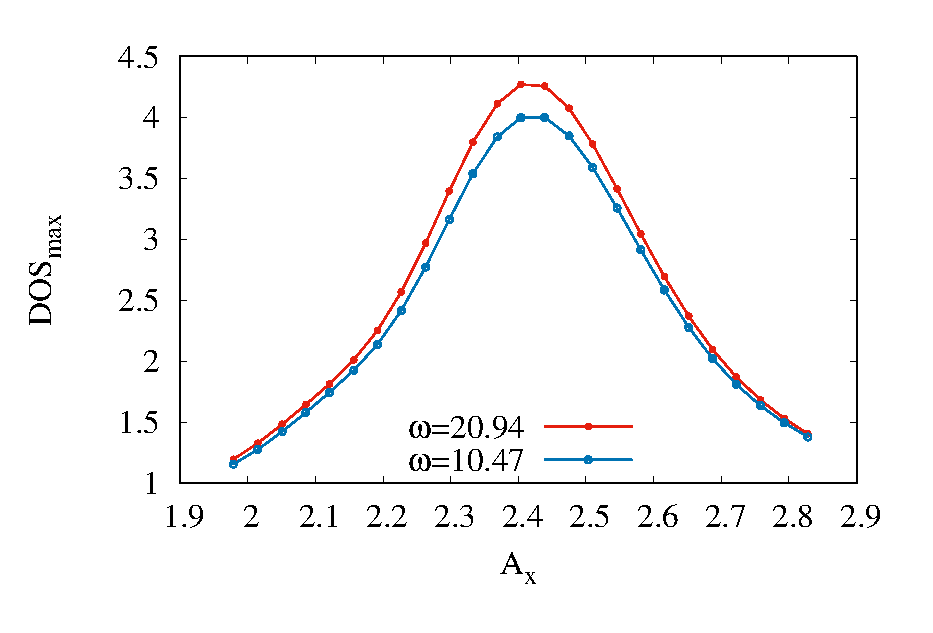
\includegraphics[width=1\linewidth]{./figure/DOS_max.eps}} \\(b)
\end{minipage}
\caption{DOS peak}
\label{fig:DOS_peak}
\end{figure}





\FloatBarrier
\section{Dispersion of doublons}



\begin{figure}[h!]
\begin{minipage}[h]{0.5\linewidth}
\center{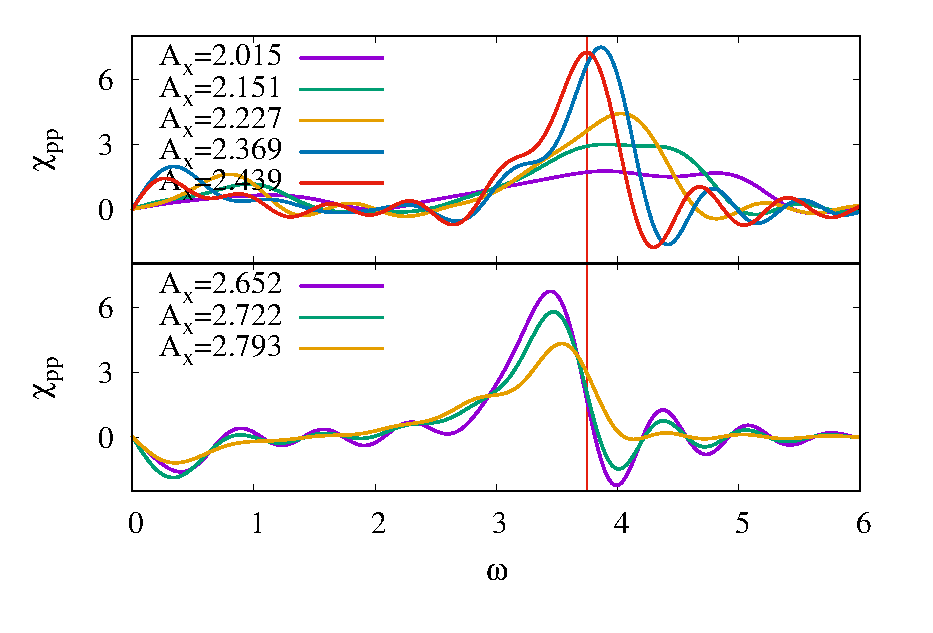
\includegraphics[width=1\linewidth]{./figure/chi_pp_loc}} (a) \\
\end{minipage}
\hfill
\begin{minipage}[h]{0.5\linewidth}
\center{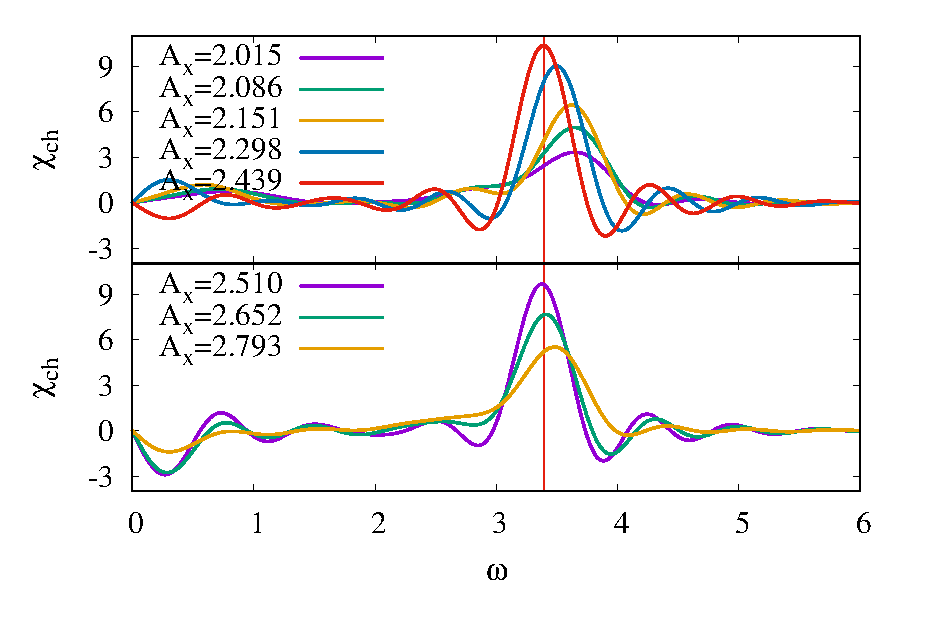
\includegraphics[width=1\linewidth]{./figure/chi_ch_loc}} \\(b)
\end{minipage}
\caption{CHI loc pp ch}
\label{fig:CHI_loc_pp_ch}
\end{figure}



\begin{figure}[h!]
\begin{minipage}[h]{0.5\linewidth}
\center{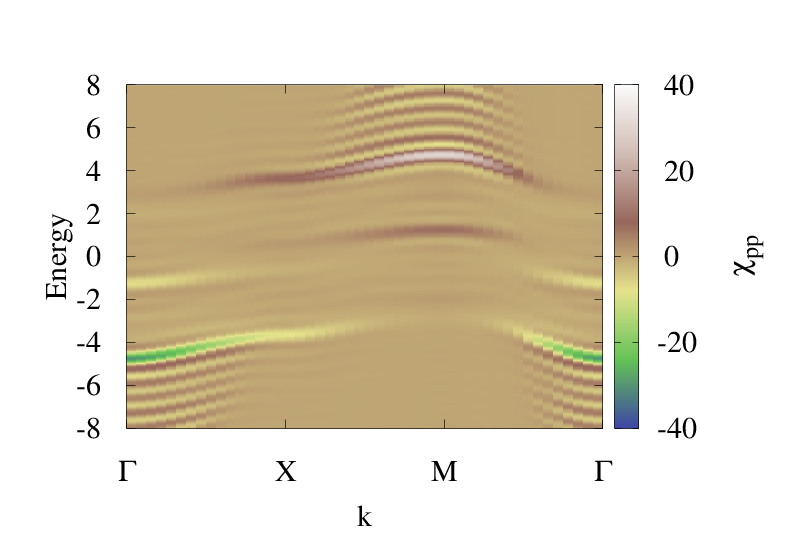
\includegraphics[width=1\linewidth]{./figure/Apic_band_pp_1275_n_05_Ax_2157.png}} (a) \\
\end{minipage}
\hfill
\begin{minipage}[h]{0.5\linewidth}
\center{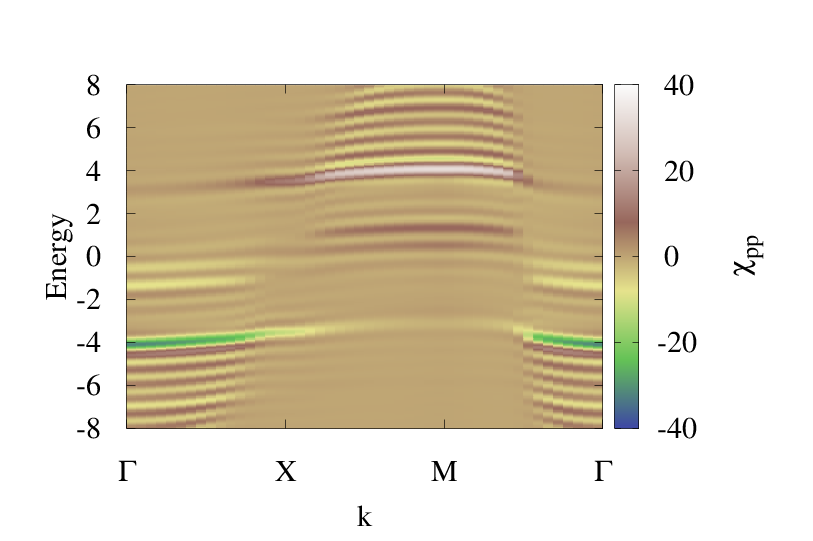
\includegraphics[width=1\linewidth]{./figure/Apic_band_pp_1275_n_05_Ax_2333.png}} \\(b)
\end{minipage}
\begin{minipage}[h]{0.5\linewidth}
\center{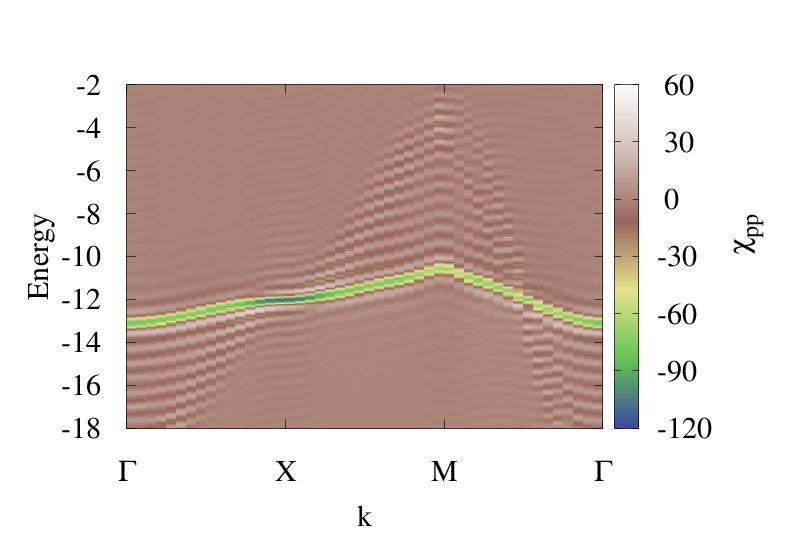
\includegraphics[width=1\linewidth]{./figure/Apic_band_pp_1275_n_1_Ax_2157.png}} (c) \\
\end{minipage}
\hfill
\begin{minipage}[h]{0.5\linewidth}
\center{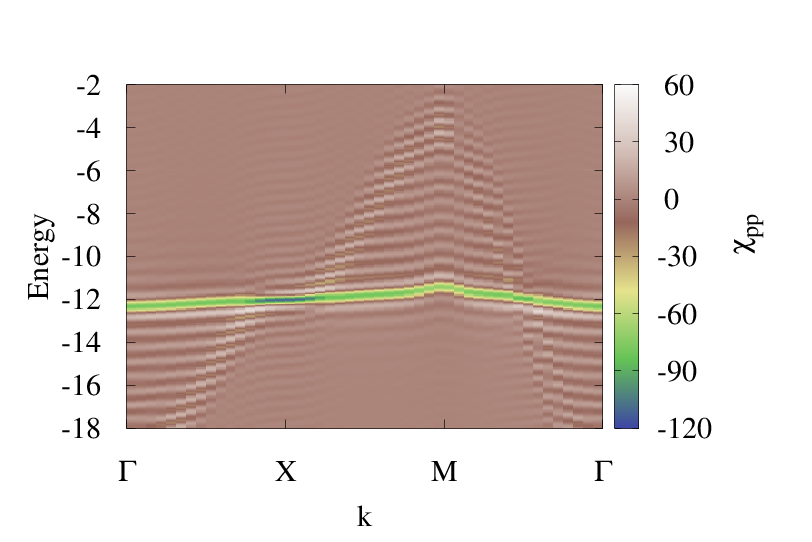
\includegraphics[width=1\linewidth]{./figure/Apic_band_pp_1275_n_1_Ax_2333.png}} \\(d)
\end{minipage}
\caption{CHI k pp. $A$-dependence. (a) $A_x=2.157$ $n=0.5$, (b) $A_x=2.333$ $n=0.5$, (c) $A_x=2.157$ $n=1$, (d) $A_x=2.333$ $n=1$.}
\label{fig:CHI_k_pp_A}
\end{figure}







\begin{figure}[h!]
\begin{minipage}[h]{0.5\linewidth}
\center{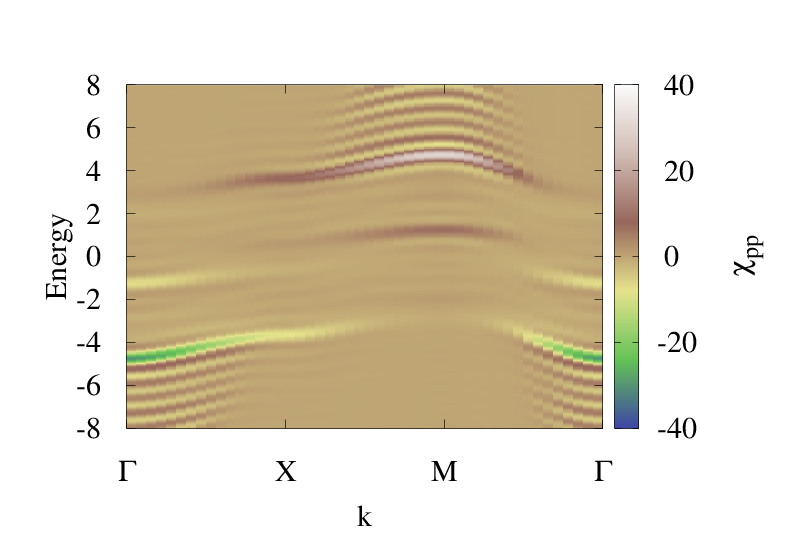
\includegraphics[width=1\linewidth]{./figure/Apic_band_pp_1275_n_05_Ax_2157.png}} (a) \\
\end{minipage}
\hfill
\begin{minipage}[h]{0.5\linewidth}
\center{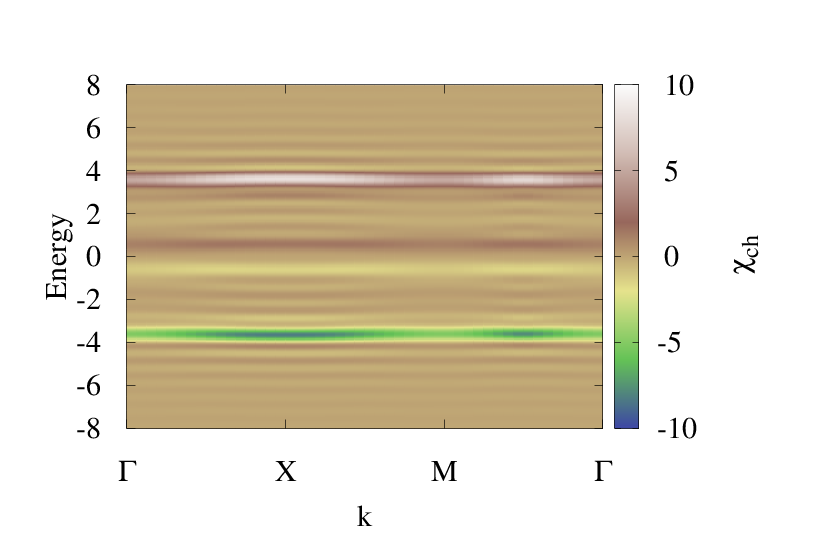
\includegraphics[width=1\linewidth]{./figure/Apic_band_ch_1275_n_05_Ax_2157.png}} \\(b)
\end{minipage}
\begin{minipage}[h]{0.5\linewidth}
\center{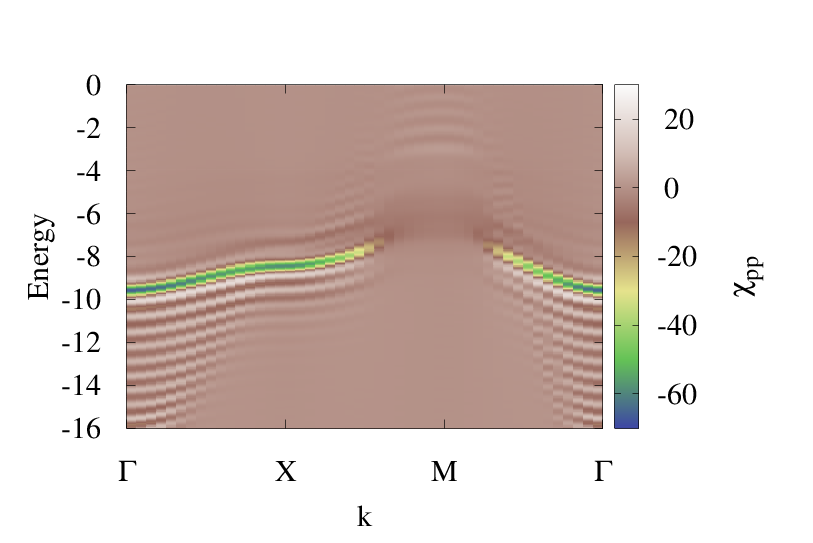
\includegraphics[width=1\linewidth]{./figure/Apic_band_pp_1275_n_0875_Ax_2157.png}} (c) \\
\end{minipage}
\hfill
\begin{minipage}[h]{0.5\linewidth}
\center{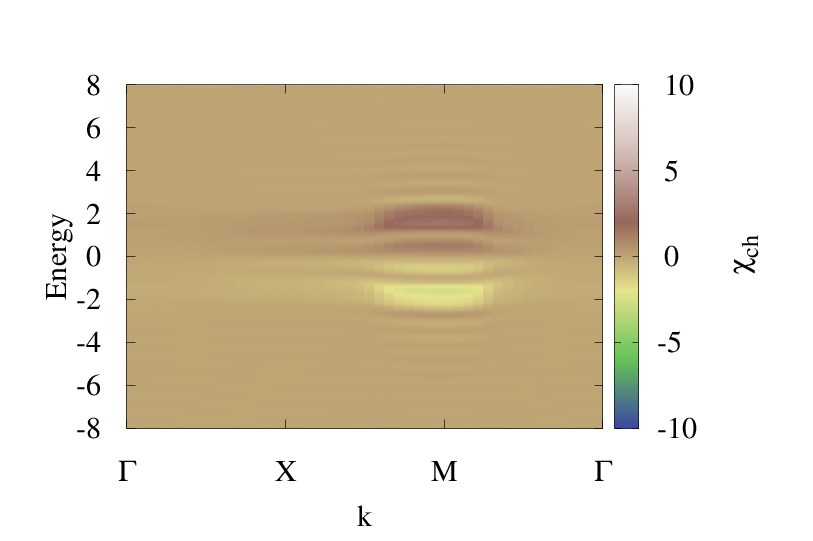
\includegraphics[width=1\linewidth]{./figure/Apic_band_ch_1275_n_0875_Ax_2157.png}} \\(d)
\end{minipage}
\begin{minipage}[h]{0.5\linewidth}
\center{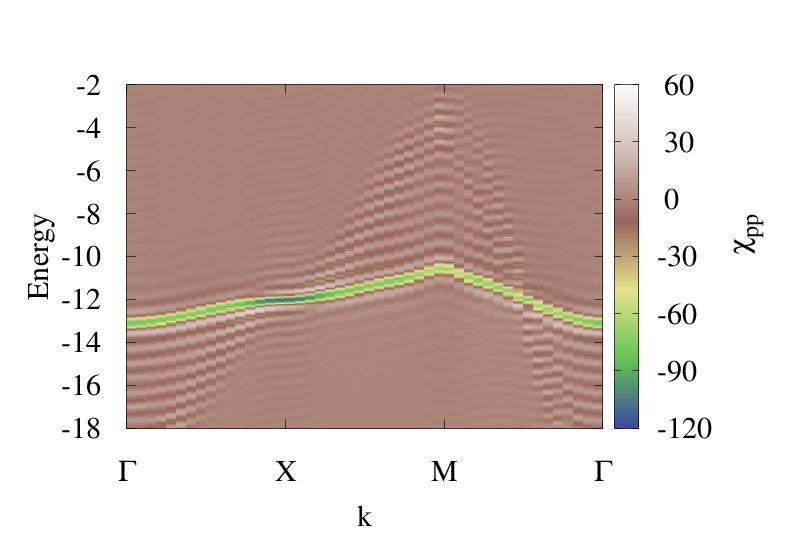
\includegraphics[width=1\linewidth]{./figure/Apic_band_pp_1275_n_1_Ax_2157.png}} (e) \\
\end{minipage}
\hfill
\begin{minipage}[h]{0.5\linewidth}
\center{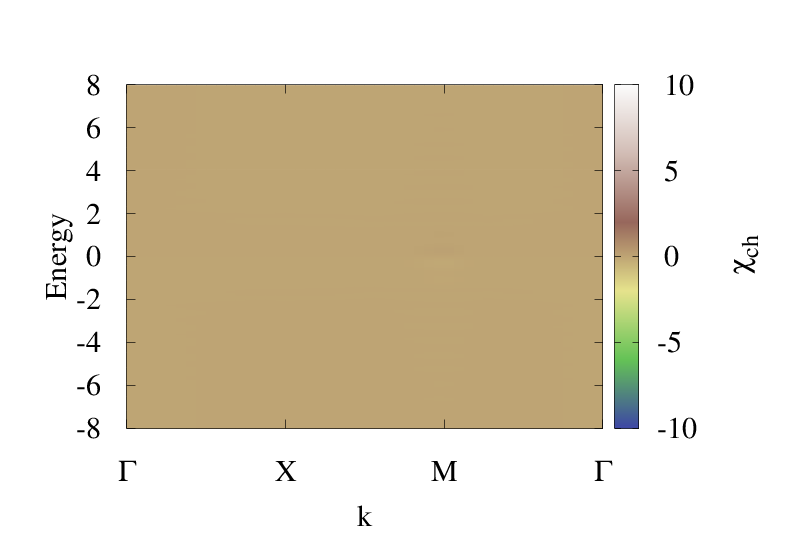
\includegraphics[width=1\linewidth]{./figure/Apic_band_ch_1275_n_1_Ax_2157.png}} \\(f)
\end{minipage}
\caption{CHI k pp. $\mu$-dependence, $A_x=2.157$. (a) $\chi_{pp}$ $n=0.5$, (b) $\chi_{ch}$ $n=0.5$, (c) $\chi_{pp}$ $n=0.875$, (d) $\chi_{ch}$ $n=0.875$, (e) $\chi_{pp}$ $n=1$, (f) $\chi_{ch}$ $n=1$.}
\label{fig:CHI_k_pp_mu}
\end{figure}






\FloatBarrier
\section{Summary}














\FloatBarrier
\clearpage
\bibliographystyle{abbrvnat}
\bibliography{references}
\end{document}
